\Chapter{Alkalmazás bemutatása}

Az alábbi fejezetben az alkalmazást fogom részletesen ismertetni a felhasználóval. Először a szerkezeti felépítését fogom bemutatni, majd kitérek minden fontosabb oldalra és a kiegészítő elemekre. Miután prezentáltam a weboldalt áttekintem miért lettek implementálva a különféle funkciók, illetve kitérek arra, hogy milyen fejlesztési lehetőségek elérhetőek a jövőben.

\section{Alkalmazás felépítése}

Az alkalmazást úgy építettem fel, hogy a látogató elsőként a Kezdőlapon találja magát. Innen lehetősége van a további három másik főoldal bármelyikére kalauzolnia magát, amennyiben szeretné (\aref{fig:draw}).

\begin{figure}[h]
\centering
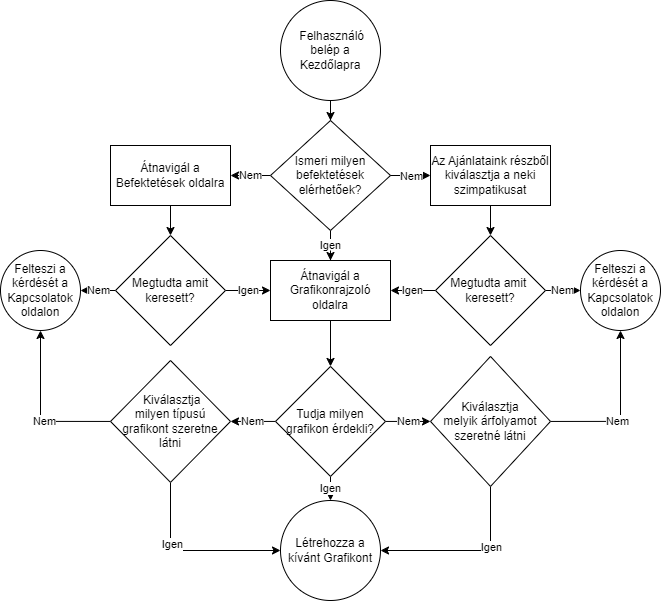
\includegraphics[scale=0.5]{images/flowchart.png}
\caption{Alkalmazás állapotdiagramja (Forrás: \cite{draw})}
\label{fig:draw}
\end{figure}

\section{Alkalmazás panelei}

Az alkalmazás megalkotásánál az alapvető szemléletem az volt, hogy szaktudásomat megjelenítéssel és funkcionalitással szeretném prezentálni. Piackutatásaim során sokat inspirálódtam különböző grafikonrajzoló weboldalakról, főként abból a szempontból, hogy milyen paneleket és oldalakat érdemes megalkotni. Következésképpen a szoftver struktúráját négy fő oldalra és hat aloldalra terveztem meg.\cite{Aegon} A főbb oldalak a következőek: 

\begin{itemize}
\item \textbf{Kezdőlap},
\item \textbf{Grafikonrajzoló},
\item \textbf{Befektetések},
\item \textbf{Kapcsolat}.
\end{itemize}

\subsection{Kezdőlap}

Minden oldalnak szüksége van egy főoldalra, nálam ezt a szerepet a Kezdőoldal tölti be. Ugyan a felhasználó a forráskód birtokában az összes többi oldalt eltudja indítani a \textbf{Live Server} akalmazásával, viszont a weboldal úgy lett felépítve, hogy az \emph{index.html} elindításával kezdjen. Ez volt az első HTML fájl amit lérehoztam és a Kezdőlapról lehet elérni egy kattintással a másik három főoldalt is.

	Minden oldalon egy általam "banner" (zászló) megnevezésű borítókép fogadja a látogatót, ezen borítókra több esetben is figyelem felkeltő szöveget írtam. A Kezdőlapon megjelenítek minden lényeges információt amit az alkalmazás kínál, továbbá lehetőség van egy kattintással átnavigálni a többi oldalra. Amit külön kiemelnék az animációk az Ajánlataink résznél, aminek a funkciója szintén a figyelemfelkeltés.

\begin{figure}[h]
\centering
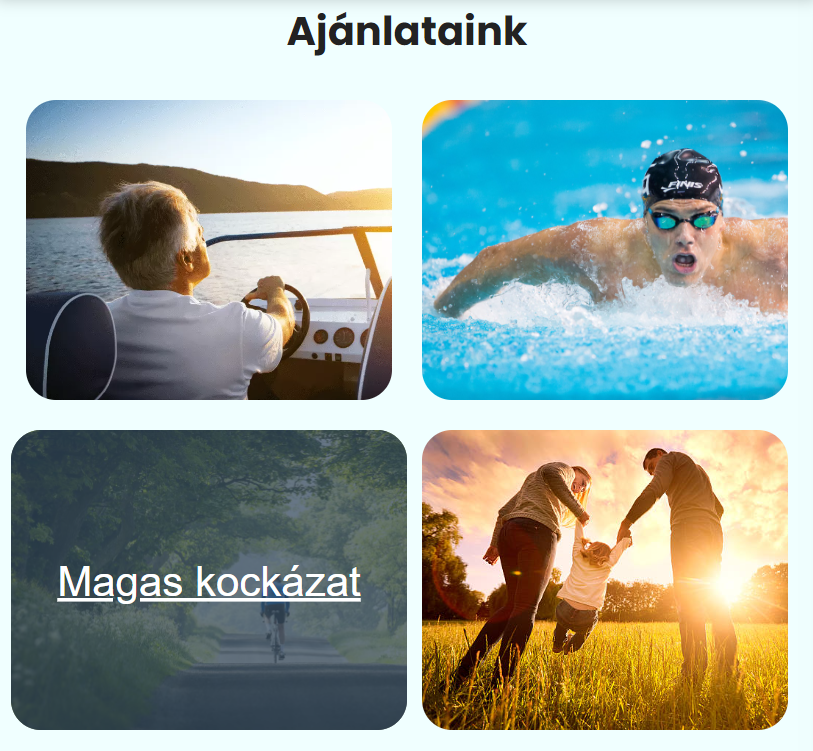
\includegraphics[scale=0.4]{images/home.png}
\caption{Kezdőlapon feltüntetett Ajánlataink részlet}
\end{figure}

\subsection{Grafikonrajzoló}

Ugyan a \textbf{Kezdőlap} hivatalosan a főoldal amivel elsőnek találkozik a látogató, mégis a szakdolgozatom fő eleme a Grafikonrajzoló oldal. A teljes projekt eköré a lehetőség köré épült, mivel a tőzsdei adatok sokasága emberi szemnek nem túl kedvező és átlátható, innen jött az ötlet, hogy az adatok perspektivikus ábrázolása sokkal jobban megfogja a célközönséget. Alapvetően a legtöbb ember vizuális beállítottságú és ezt a pszichológia tényt használtam fel a grafikonrajzoló megtervezésénél.

	Megvalósítását tekintve a borítókép is egyértelműen jelzi, hogy az oldalon gráfokkal lehet találkozni. Ezek után egy kisebb bevezető szöveg következik, ami ismerteti hogyan lehet akkurátusan leolvasni a megjelenített adatokat. Természetesen a megjelenítés felépítése nem tér el az átlagtól, így akinek ez lenne a legelső ilyen témájú weboldal, sem fogja magát elveszve érezni, hiszen a tankönyvek, hirdetések és a közmédia is ezen ábrázolást használja, amely információhalmazzal nagy valószínűséggel találkozott a felhasználó élete során. Ha mégsem így lenne, akkor eljött a megfelelő alkalom az alkalmazásom személyében.

	Funkcionalitása úgy épül fel, hogy elsőnek lehetőségünk van kiválasztani milyen fajta gráfot szeretnénk látni. Ötféle opció áll rendelkezésre amelyeket már korábban ismertettem a második fejezet \textbf{Grafikonok története és típusai} részben. Mivel a vonaldiagram a legelterjedtebb gráf, így alapértelmezetten az került kiválasztásra, ha a felhasználó nem változtat az opción, akkor aképpen jelenik meg a gráf. 

Következő adatsor a befektetési alapok. Jelenleg hat különböző típusú befektetési alap közül lehet választani, amiket a \emph{Befektetések} alfejezetben fogok ismertetni. Hogy ne legyen túl sok adat egyszerre megjelenítve korlátoztam a választási lehetőségeket, miszerint egyszerre csak egyféle alapot lehet választani. 

Végül a tőzsdei árfolyamok következnek amiket szintén ismertettem a második fejezet  \textbf{Tőzsdei árfolyami} cikkében. Szintén ötféle választási lehetőség tárul a felhasználó elé, amelyek közül az egyszerű átlátás végett egyet lehet választani.

\begin{figure}[h]
\centering
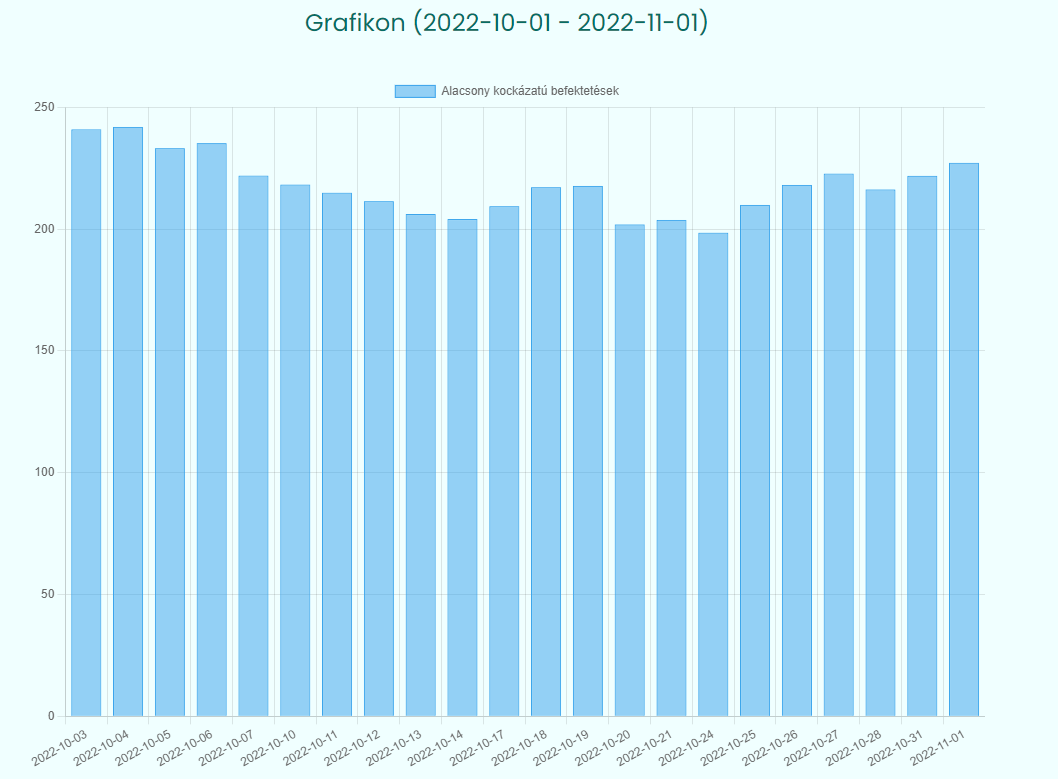
\includegraphics[scale=0.4]{images/graphPlotter.png}
\caption{Grafikonrajzoló által készített gráf példa}
\end{figure}

\subsection{Befektetések}

A Befektetések oldalnak a fő paradigmája az információ közlése és ismertetése. Az \textbf{Az Elméleti háttér} fejezetben már taglaltam, hogy a tőzsde és a befektetések elrettentő szavak azon személyeknek akiknek nincs átfogó gazdasági szakértelme, így ez az oldal azt a célt szolgálja, hogy bárki tudását gyarapíthassa. Jelenleg az oldalamon hat különböző befektetés elérhető, mindegyik befektetéshez külön aloldal tartozik, ahol részletes leírás, táblázat és éves nettó értékelés is található. Felépítését tekintve, hogy jobban meglehessen őket jegyezni mindegyik befektetés kapott saját borítóképet és fantázia nevet. A befektetések leírása általam készített kreáció amiket a fő inspirációként szolgáló \textbf{Aegon Biztosító Zrt.} hivatalos weboldaláról szereztem \cite{Aegon}. Mindegyik befektetés adathalmaza valós részvények adatait képezik, mint például a \emph{Tempó 2 Andante} alaphoz a Google részvényein alapszik. Ezen adatokat a már korábban említett EOD oldalról gyűjtöttem össze API hívásokat alkalmazva. \cite{eod} 
A Befektetések oldalon található hat befektetési alap:
\begin{itemize}
\item \textbf{Tempó 2 Andante (Alacsony kockázatú befektetés)},
\item \textbf{Tempó 5 Moderato (Közepes kockázatú befektetés)},
\item \textbf{Tempó 8 Allegro (Magas kockázatú befektetés)},
\item \textbf{Abszolút hozamú befektetési alap (Családi csomag)},
\item \textbf{Feltörekvő Európa Kötvény befektetési alap (Európai portfólió)},
\item \textbf{Megatrend Részvény befektetési alap (Megújuló energia)}. \cite{Aegon}
\end{itemize}

\begin{figure}[h]
\centering
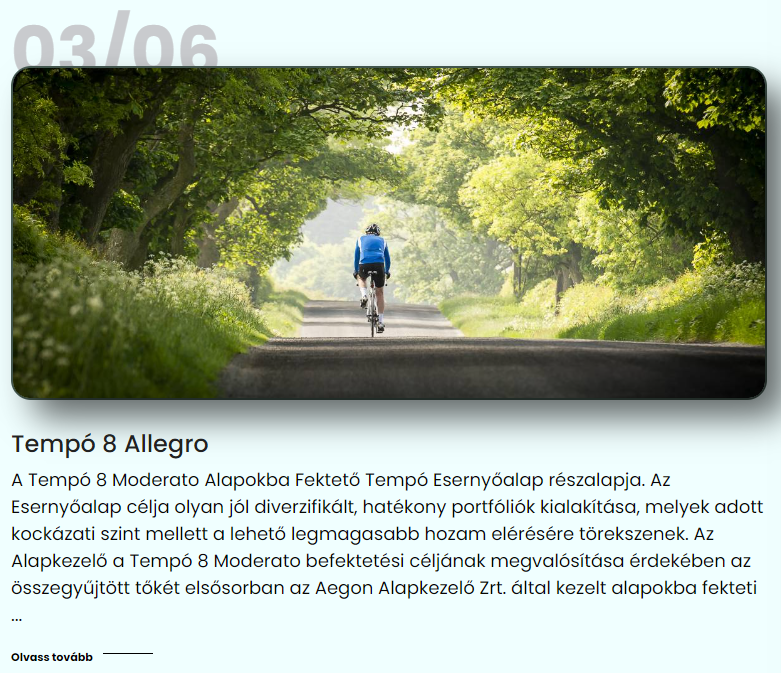
\includegraphics[scale=0.5]{images/invest.png}
\caption{A hat befektetési alap közül a harmadik.}
\end{figure}

\subsection{Kapcsolat}

Amikor a fejlesztési stratégiám még a tervezési fázisban (\aref{fig:planning}) járt, akkor nem fordítottam nagyobb figyelmet erre a panelre, mert nem tartottam fontosnak. Viszont a konzulensem által is erősen javasolt piackutatási folyamat során meglepő információra bukkantam. A legtöbb blogban és elemzésben elengedhetetlen elemnek tartják a \textbf{Kapcsolat} oldalt. "A kapcsolati adatok könnyű megtalálása az egyik legfontosabb dolog, hogy a weboldalad megbízhatóvá váljon. Az email, telefon vagy élő chat elérésedet helyezd el minden aloldalon."  \cite{contact}. Tehát kétség sem fér hozzá, hogy az oldal kötelező eleme legyen az alkalmazásomnak, viszont felmerült bennem a kérdés, hogy mégis milyen módon állítsam össze? 

	Nos erre a kérdésre hamar megtaláltam a választ, a Kapcsolat oldal kivitelezését aszerint fogom megalkotni, mint ahogy egy felhasználó elvárná. Elsőként kiválasztottam egy figyelemfelkeltő és megragadó képet ami egyértelműen szimbolizálja milyen elemek találhatóak. Továbbiakban arra fókuszáltam, hogy a látogató számára minden olyan szükséges metaadatok (\aref{fig:contact}) jelenjenek meg amivel kapcsolatba lehet lépni velem. A Kapcsolat címmel ellátott blokkban megadtam a "Fő iroda" adatait, amiket a Font Awsome által kiválasztott ismerős ikonokkal jeleztem. Kiegészítettem még egy beszúrt élő Google térképpel, ami az iroda "központját" célszerű mutatni, illetve elhelyeztem még egy üzenet küldő formot, ha bármilyen kérdés felmerülne a felhasználóban.

\begin{figure}[h]
\centering
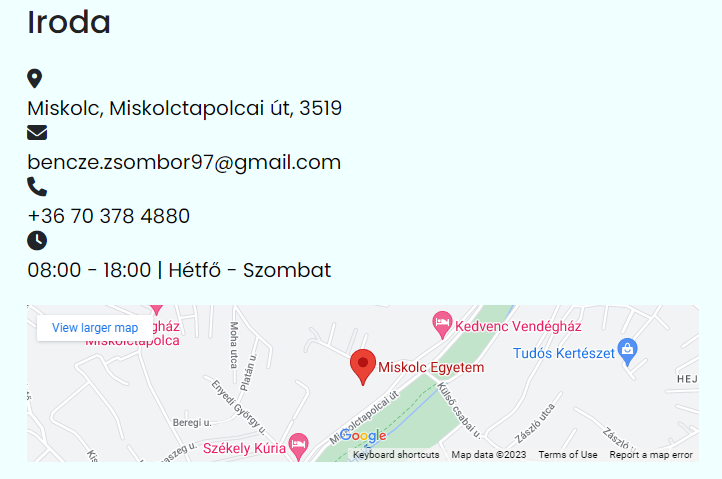
\includegraphics[scale=0.5]{images/contact.png}
\caption{Részlet a kapcsolat oldalról}
\label{fig:contact}
\end{figure}


\subsection{Design megtervezése}

Először felmértem, hogy mely oldalak lesznek a weboldalam legfontosabb elemei, majd úgy alakítottam ki a szerkezetüket, hogy egységesen passzoljon mindegyikre. Témának zöldes-kékes színvilágot választottam, ezért lett égszínkék a háttérszín. A szövegek színe megmaradt a fekete és annak árnyalatainak, mint például: \emph{\#222} RGB kódú világosabb feketeszín. Továbbá a gombok és feliratok zöldes színt kaptak, amihez a leggyakrabban használt \emph{\#088178} RGB kódú látványt használtam.

\subsection{Navigáció}

A navigációt úgy terveztem meg, hogy a fő oldalak között bármikor lehessen általa váltani. Mindig a képernyő tetején helyezkedik el és követi annak mozgatását, így a navigálás felhasználó barát és könnyed. Ha a képernyő pikszel mérete kisebb a monitorénál, akkor vízszintes helyezkedését függőleges váltja fel, amit egy gomb megnyomásával lehet előhozni és elrejteni.

	A weboldalakon kétféle menürendszer használatos: vízszintes és függőleges. (\aref{fig:navbar})

\begin{figure}[h]
\centering
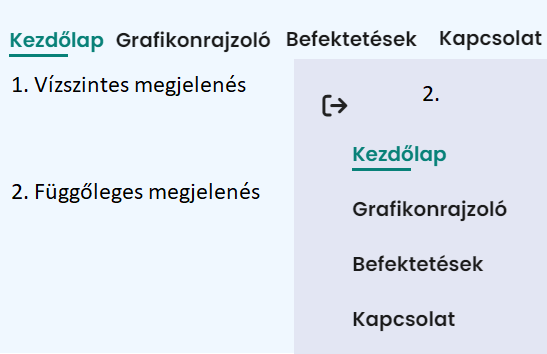
\includegraphics[scale=0.5]{images/navbar.png}
\caption{Navigációs sáv két típusú megjelenítése}
\label{fig:navbar}
\end{figure}

\subsection{Lábléc}

"Talán furcsán hangzik, de minden weboldal egyik legfontosabb eleme a lábléc" \cite{contact}. Biztos, hogy nem ez a legfigyelemre méltóbb alkotóeleme a weboldalamnak, viszont ez az a hely amit a látogató felkereshet, ha információra van szüksége.

\begin{figure}[h]
\centering
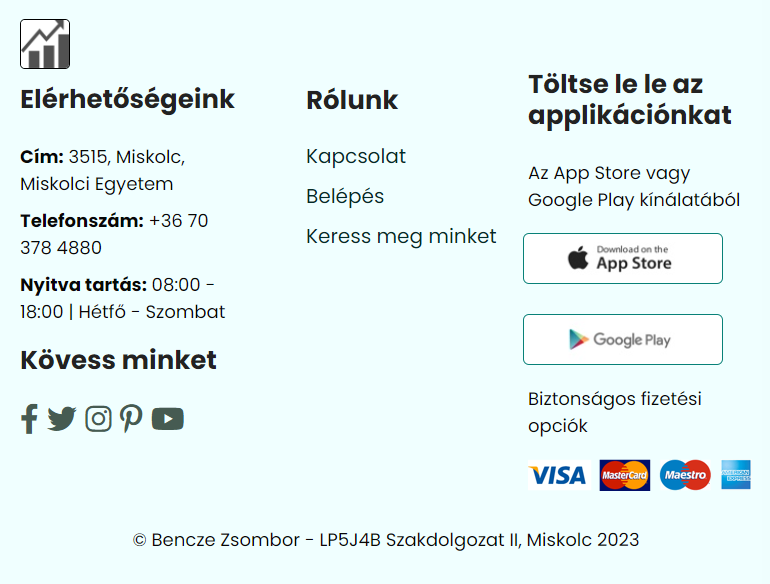
\includegraphics[scale=0.5]{images/footer.png}
\caption{Lábléc}
\end{figure}

\subsection{Logó}

A logó az alkalmazás bal oldalán helyezkedik el, mind a navigációs sávon, mind a láblécen. A logóra kattinva bármely oldalról eljuthat a felhasználó a Kezdőlapra. A logó megjelenését én készítettem, a dizájn célja az volt, hogy a látogató számára egyértelműen mutassa, ez egy részvényekkel foglalkozó weboldal.

\section{Alkalmazás áttekintése}

Ebben a szekvenciában szubjektív módon szeretném bemutatni, mi indokolta a weboldalam létrejöttét. Olyan szempontokat fogok felsorolni amik az én alkalmazásomban megtalálhatóak, de más általam felmért weboldalakban hiányoltam.

\subsection{Más oldalakkal összehasonlítás}

Ahogy már említettem a lista teljesen szubjektív és az oldalon található funkciókat szeretném megindokolni, hogy miért lettek lefejlesztve és mi volt velük a célom. \\

\textbf{Ami az én oldalalom megtalálható}:

\begin{itemize}
\item Könnyű navigálás, hiszen a főoldalról is elérhető bármelyik oldal, illetve a navigációs sáv követi a képernyő mozgását. 
\item Képpekkel ellátott befektetések, hogy befogadhatóbbak legyenek.
\item Többfajta diagram típus közül lehet választani.
\item Többféle árfolyam is választható.
\end{itemize}

\textbf{Ami az én oldalalom nem található}:

\begin{itemize}
\item Vonaldiagramnál több gráf választható,
\item Bejelentkezési felület,
\item Nyelvesítés,
\item Adatok letöltése.
\end{itemize}

\subsection {Miért fontosak a tőzsdét elemző weboldalak?}

A tőzsdére történő befektetés jövedelmező vállalkozás lehet, de alapos kutatást és elemzést igényel a megalapozott döntések meghozatalához. Az egyik értékes erőforrás, amely jelentősen segítheti a befektetőket a döntéshozatali folyamatban, a grafikonrajzoló weboldalak. Átfogó adatvizsgálat, pénzügyi kimutatásokhoz és iparági betekintésekhez szokás használni. A tőzsde rendkívül dinamikus, az árfolyamok különböző tényezők miatt gyorsan ingadoznak. A grafikonrajzolók segítségével folyamatosan figyelemmel kísérhetőek a piaci viszonyok, és azonnali betekintés nyerhető.
A technológiai fejlődésnek és a különféle platformok elérhetőségének köszönhetően minden eddiginél egyszerűbb megtalálni a releváns befektetéseket.

\subsection{Hogyan lehet felhasználni adatok elemzéséhez?}

A grafikon gyakori módszer az adatok összefüggéseinek vizuális szemléltetésére. A grafikon célja, hogy olyan adatokat mutasson be, amelyek túl sok vagy bonyolult ahhoz, hogy a szövegben és kisebb helyen megfelelően leírhatók legyenek. Ha az adatok kifejezett trendeket mutatnak, vagy a változók közötti kapcsolatokat tárják fel, grafikont kell használni. 
A gráfokon használt egyik gyakori elemzési technika a \textbf{részvényelemzés}.

\subsection{Részvényelemzés}

A részvényelemzés népszerű a technikai elemzés, a múltbeli részvényárfolyam-
tevékenységre támaszkodva a jövőbeli árfolyamtevékenység előrejelzésében. Gyakori módszer a befektetők és kereskedők számára vételi és eladási döntések meghozatalára. A múltbeli és jelenlegi adatok tanulmányozásával és értékelésével a befektetők és a kereskedők megalapozott döntések meghozatalával próbálnak előnyt szerezni a piacokon. Az alábbiakban tárgyalt elsődleges módszerekben a befektetők pénzügyi kimutatásokat, részvényárfolyamokat, piaci mutatókat vagy iparági trendeket használnak befektetési döntéseik meghozatalához. \cite{investo}
